\begin{center}
    \textbf{--------- Lezione 1 - 3 marzo 2021 ---------}
\end{center}

\begin{comment}
\section{Distributed System and Pervasive Computing}
\end{comment}


\textit{Un sistema distribuito è una collezione di computer indipendenti (nodi collegati, che possono comunicare tra loro) che appare ai suoi utenti come un singolo sistema coerente.}

I nodi non sono solo indipendenti ma anche collegati tra loro (non hanno quindi una memoria condivisa e sono collegati in qualche modo). 
\begin{figure}[!ht]
    \centering
    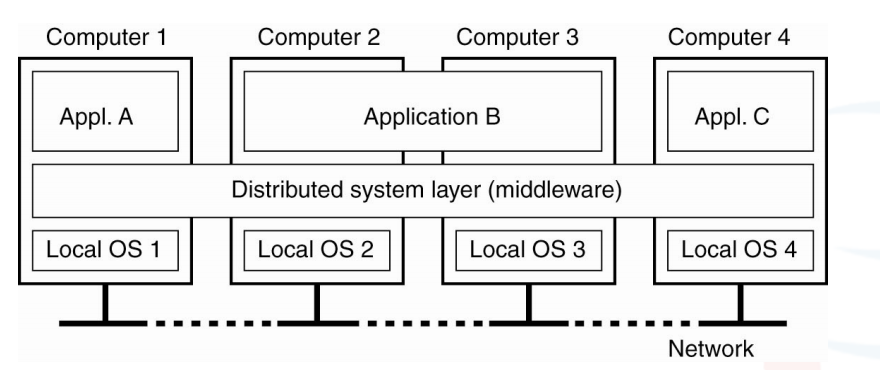
\includegraphics[width = .8\textwidth]{images/lezione1/architettura sd.PNG}
\end{figure}

Dal punto di vista architetturale abbiamo una collezione di PC, ognuno ha un local OS (sistema operativo) e ognuno ha applicazioni che vuol far girare. C'è poi uno strato che permette di far collaborare i vari PC che si chiama middleware, il quale mette a disposizione alle applicazioni la stessa interfaccia.\\

Si sviluppa un software ad un certo livello che permette di andare a nascondere agli utenti finali gli n computer e farli apparire come se fosse un sistema unico. \\

\newpage
Esempi: 
\begin{itemize}
    \item se abbiamo un insieme di PC in rete e un file system condiviso, non solo i file sono condivisi ma anche le risorse di calcolo
    \item nei multiplayer online games, chi gioca non deve sapere dove lo stato del gioco viene memorizzato
    \item WWW sistema distribuito che si occupa della gestione distribuita di documenti identificati univocamente con URL. Il web non è esattamente un sistema distribuito. Attraverso l'URL si capisce dove si trova il documento, la trasparenza, quindi, è svanita. \\
    In un sistema distribuito vero devo avere identificatori di risorse che non danno informazioni sulla locazione dei documenti.
\end{itemize}.
Lamport, l'inventore di latex, dice "You know you have one when the crash of a computer you've never heard of stops you from getting any work done".
Significa che se abbiamo un problema è difficile capire cos'è successo perché in un sistema distribuito è difficile effettuare il debugging. 


\chapter{Obiettivi di un sistema distribuito}

\section{Accessibilità}
Un sistema distribuito deve rendere accessibili le sue risorse.

\section{Trasparenza}
Ci sono diversi tipi di trasparenza: 
\begin{itemize}
    \item Accesso: nasconde differenze di filesystem e/o come sono rappresentati i dati e come viene effettuato l'accesso ad essi. Esempio: considerando i 4 pc che fanno parte del sistema, voglio far risultare trasparente un accesso ad un file condiviso. Ogni PC però ha un file system diverso (esempio uno EXT4 per Linux, NTFS per Windows...).
    \item Locazione: non devo sapere dove si trova la risorsa
    \item Migrazione: nasconde che la risorsa potrebbe spostarsi
    \item Rilocazione: nasconde che la risorsa potrebbe spostarsi durante l'utilizzo
    \item Replicazione: nasconde quando una risorsa viene replicata. Questo viene fatto per ridondanza (sopperiamo a eventuali mal funzionamenti) ed efficienza. 
    \item Concorrenza: nascondere che una risorsa potrebbe essere condivisa da molti utenti che eseguono modifiche in maniera concorrente
    \item Failure: il sistema deve nascondere eventuali fallimenti e ripristinare automaticamente la risorsa 
\end{itemize}

\section{Apertura (Openess)}
Un sistema aperto dovrebbe offrire:
\begin{itemize}
    \item interoperabilità
    \item portabilità
    \item estensibilità
\end{itemize}

L'apertura può essere raggiunta attraverso:
\begin{itemize}
    \item l'utilizzo di protocolli standard
    \item pubblicazione di interfacce chiave
    \item testing e verifica della conformità dei componenti rispetto a determinati standard
\end{itemize}

\section{Scalabilità} 
La scalabilità è una caratteristica fondamentale in un sistema distribuito di larga scala. Quello che vogliamo ottenere è che più il sistema è grande (e viene ampliato) più è performante. Bisogna dunque evitare centralizzazione di servizi, dati e algoritmi.\\

Ci sono diversi problemi in cui si incorre quando si cerca di ottenere la scalabilità: 
\begin{itemize}
    \item centralizzazione dei servizi: singolo server per tutti gli utenti. Esempio: il bonus bici dove si ha un unico server per più utenti e dove la risorsa stava nello stesso posto. Tutti gli utenti nello stesso momento hanno cercato di accedere a quella risorsa.
    \item centralizzazione dei dati. Esempio: un singolo elenco telefonico on-line 
    \item centralizzazione degli algoritmi: routing basato su tutte le informazioni.
\end{itemize}

Le caratteristiche degli algoritmi decentralizzati: 
\begin{itemize}
    \item nessuna macchina (nodo) dispone di informazioni complete sullo stato del sistema
    \item le macchine prendono decisioni basate solo su informazioni locali
    \item il guasto di una macchina non rovina l'algoritmo
    \item non esiste l'assunzione di avere un clock globale. Non è possibile coordinare gli orologi sulle macchine, infatti non sono mai sincronizzati perfettamente
\end{itemize}

\textit{In un contesto client server come faccio a rendere scalabile un sistema?} \\Si può delegare del lavoro al client, in modo che aggiungendo client (scalabilità) il lavoro del server aumenti ma sia comunque gestibile (poichè abbiamo scaricato del lavoro sul client).\\
\begin{center}
    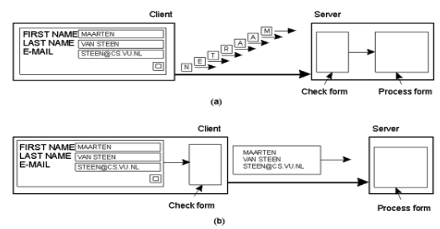
\includegraphics[width = .8\textwidth]{images/lezione1/Scaling.png}
\end{center}
Un sistema distribuito che usiamo tutti i giorni è il DNS. 
Quando lanciamo un indirizzo simbolico, prima che il browser vada a fare la richiesta web viene interrogato il DNS, si guarda nella cache,  si guarda nel name server che abbiamo ma se quello non è in grado di risolverlo, allora si interrogano altri nodi.
Questa procedura è del tutto trasparente. 


\subsection{Insidie}
Quando si sviluppa un sistema distribuito si possono effettuare delle valutazioni errate come:
\begin{itemize}
    \item la rete è affidabile
    \item la rete è sicura 
    \item la rete è omogenea
    \item la topologia non cambia
    \item la latenza è zero
    \item la larghezza di banda è infinita
    \item il costo di trasporto è zero
    \item c'è un amministratore
    \item il debug delle applicazioni distribuite è analogo alle applicazioni standard
\end{itemize} 

\section{Tipi di sistemi distribuiti}
\begin{itemize}
    \item Distributed Computing Systems: 
    \begin{itemize}
        \item cluster
        \item cloud computing
        \item edge computing
    \end{itemize}
    \item Distributed Information Systems:
    \begin{itemize}
        \item database distribuiti
        \item transazioni distribuite
    \end{itemize}
    \item Distributed Pervasive Systems
\end{itemize}

\subsection{Distributed Computing Systems}
\subsubsection{Cluster}
I cluster sono utilizzati dai principali fornitori cloud. \\
Un cluster è una collezione di server uguali o simili strettamente connessi da una rete locale ad alta velocità che solitamente hanno lo stesso sistema operativo.\\
Gli obiettivi principali sono: avere un'attività di elaborazione ad alte prestazioni (distribuisce il calcolo su più nodi) e avere un'alta disponibilità (se un sistema va offline, fornisce comunque la richiesta). \\
Ci sono due tipi di cluster:
\begin{itemize}
    \item asimmetrico: è il più utilizzato, qualche nodo ha un ruolo principale (nodo master) rispetto ad altri e ha il compito di distribuire i task ad un insieme di nodi di computazione. \\
    Esempi: Google Borg, sistema utilizzato internamente da Google per gestire i suoi cluster e Beowulf analogo per Linux.
    \begin{center}
    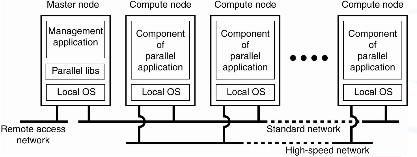
\includegraphics[width = .8\textwidth]{images/lezione1/ClusterAsimm.png}
    \end{center}
    Ciascun nodo ha un local OS. I nodi sono collegati da high-speed network oltre che attraverso una normale rete.\\Il cluster verrà raggiunto dall'esterno attraverso remote access network. \\Questi nodi sono tutti uguali, tranne il master che ha un applicazione di management per distribuire il workload sui nodi.
    \item simmetrici: non c'è un master, tutti i nodi sono allo stesso livello e hanno lo stesso software installato. Questi nodi devono auto-organizzarsi per distribuire il carico e fornire le stesse funzionalità in qualche modo.\\ Esempio: MOSIX, che ha molteplici versioni, che in ambito Linux permette di realizzare cluster simmetrico.
\end{itemize}


\subsubsection{Caso di Borg}
\begin{center}
    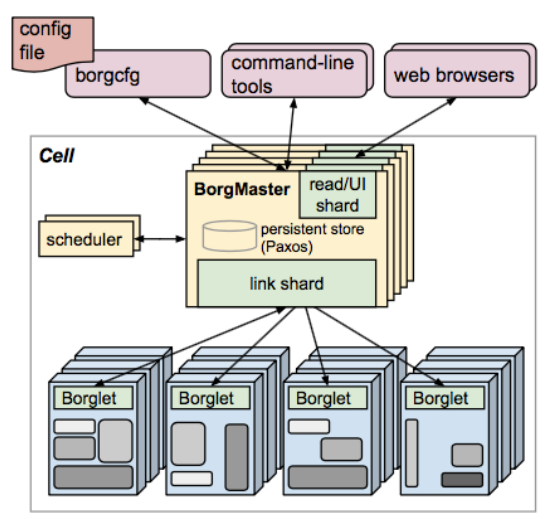
\includegraphics[width = .5\textwidth]{images/lezione1/borg.PNG}
\end{center}

Ci sono il nodo master (Borg master) e i nodi slave (Borglet) che non sono come il nodo master. I Borglet eseguono parti di applicazioni che vengono scaricati sui nodi che partecipano (slave) in modo tale che venga distribuita la computazione.\\
Il master può essere o non essere collegato ad high speed network, poiché la comunicazione più frequente avviene tra i nodi ed è li che si vuole ottimizzare.\\
Possiamo notare dallo schema che BorgMaster è replicato. Questo perché altrimenti se andasse giù il master si bloccherebbe tutto. I dati fondamentali di cui ha bisogno il master per operare vengono condivisi sulle copie attraverso uno storage distribuito e Paxos garantisce che tutti abbiano la stessa visione sullo stato del sistema.\\\

Da Borg ha preso ispirazione Kubernetes, un sistema di gestione di cluster più sofisticato (sviluppato da Google), che viene utilizzato principalmente in ambienti conteinerizzati. Google ha donato questo sistema alla Linux Foundation ed è quindi open source. 
\begin{center}
    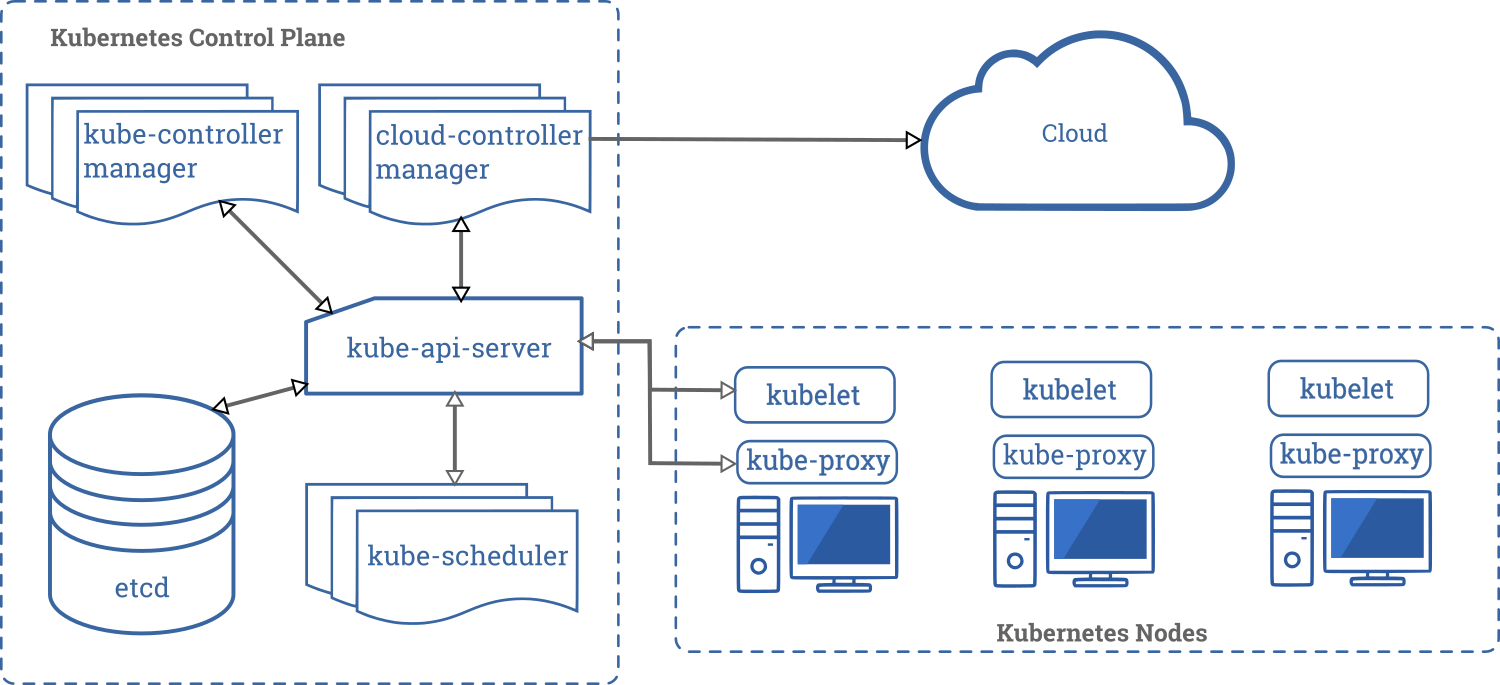
\includegraphics[width = .8\textwidth]{images/lezione1/kubernetes.png}
\end{center}
Etcd è un database chiave valore. Borglet - Kubelet.

\subsubsection{Cloud computing}
Il cluster assume che le macchine siano localizzate nello stesso posto, per essere collegate ad una rete ad alta velocità.\\ Un'infrastruttura cloud invece prevede anche una distribuzione geografica. Le macchine saranno quindi collegate tra loro con canali che utilizzato internet.\\
Il cloud computer è un modello accessibile in qualunque momento e conveniente che può essere rapidamente fornito e rilasciato con un minimo di sforzo di gestione o interazione con il fornitore di servizi.

\subsubsection{Caratteristiche cloud}
\begin{itemize}
    \item i nodi sono eterogenei: nei cluster spesso le macchine sono identiche. Nel cloud i nodi possono essere invece molto eterogenei a livello di hardware e a livello di software
    \item le connessioni di rete sono eterogenee nelle loro capacità e affidabilità 
    \item on-demand self-service: riconfigurare le risorse ad un certo utente in modo semplice
    \item ampio accesso alla rete: capacità del cloud sono disponibili su tutta la rete accedute da meccanismi standard (trasparenza rispetto all'accesso) tramite API.
    \item pool di risorse: le risorse di elaborazione del provider vengono raggruppate per servire più consumatori
    \item rapida elasticità: le funzionalità e le risorse possono essere fornite in modo elastico (dare o restituire rapidamente)
    \item servizio misurato: chi implementa un cloud deve implementare dei sistemi di misura. Esempio: quanta ram ho usato?

\end{itemize}


\subsubsection{Cloud service models}
\begin{itemize}
    \item SaaS: un utente inesperto si appoggia ad un sw fornito dal cloud, ad esempio google docs.
    \item Paas: una via di mezzo tra IaaS (ho bisogno una macchina, non la voglio comprare ma voglio autonomia su quello che posso installarci, voglio soltanto l'infrastruttura) e SaaS. L'applicazione finale la voglio sviluppare io, però voglio utilizzare db ad alto parallelismo/disponibilità che mi viene fornito. Quindi uso quello del cloud. 
    \item Iaas: sviluppare ed eseguire un software su un'infrastruttura cloud arbitraria 
\end{itemize}


\subsubsection{Cloud Deployment Models}
\begin{itemize}
    \item private cloud: utilizzato da una singola organizzazione composta da più consumatori, ad esempio l'università di Milano
    \item community cloud: utilizzato da una specifica comunità di consumatori provenienti da organizzazioni che condividono interessi
    \item public cloud: uso aperto da parte del pubblico in generale, ad esempio Amazon e Microsoft
    \item hybrid cloud: posso avere sia dati pubblici che privati. Faccio quindi una soluzione ibrida in maniera da integrare, mantenendo un certa località dei dati e controllo di accesso.
\end{itemize}

\subsubsection{Cloud Computing Infrastructure}
Switch per gestire una rete ad altà velocità e tecnologie di load balancing con hardware e software molto sofisticati.\\
Ogni data center ha uno o più cluster di migliaia di nodi collegati tra loro.

\subsubsection{Edge (Fog) computing}
IOT: dispositivi connessi (possono far parte di sistemi disribuiti) spesso con sensori che producono enormi quantità di dati, alcuni dei quali devono essere processati in tempo reale. Quindi la latenza introdotta dal cloud in molti casi si rivela un problema. \\
L'idea è di avere una struttura gerarchica (anzichè solo cluster dislocati del mondo), in cui abbiamo server vicini a dove i dati vengono prodotti (edge, confine della rete) e questi nodi riescono a connettersi con i dispositivi che producono questi dati e quindi fare processing o preprocessing in tempo reale, in un modo che il cloud generico non riuscerebbe a fare.
5G ha un ruolo chiave in questo ambito, ma da solo non riesce. \\
I dispositivi di edge possono essere di tipo diverso, ma sostanzialmente sono un primo passaggio da IoT e sensori verso il cloud. \\
Fog viene usato spesso come sinomino, ma a volte viene utilizzato in maniera differente per indicare i livelli di decentralizzazione in gerarchie a più di 3 livelli (?).

\begin{comment}
\subsection{Distribuited Information Systems}
\subsubsection{Sistemi transazionali}
La caratteristica principale di una transazione è che vengono eseguite tutte le operazioni o nessuna di loro. Le operazioni in base alle transazioni possono essere chiamate di sistema, procedure di librerie o blocchi di istruzioni in un linguaggio.
Nei sistemi transazionali valgono le proprietà ACID:
\begin{itemize}
    \item atomicità: consiste nel riuscire ad eseguire tutto un blocco di istruzioni, o non eseguire nulla in caso contrario
    \item consistenza: quando inizia una transazione il database si trova in uno stato coerente e quando la transazione termina, il database, dev'essere in uno stato coerente (non si devono verificare contraddizioni)
    \item isolamento: ogni transazione deve essere eseguita in modo isolato e indipendente dalle altre transazioni
    \item durabilità: una volta che la transazione ha reso effettiva la modifica esse sono permanenti
\end{itemize}

\subsubsection{Enterprise Application Integration (EAI)}
La comunicazione tra le diverse applicazioni del sistema avviene senza rcorrere a transazioni sui DB. Si utilizza un livello middleware, tra client e server, che gestisce le comunicazioni tra i diversi componenti del sistema utilizzando RPC, RMI e messaggi.
\end{comment}

\subsection{Distribuited Pervasive Systems}
L'idea generale è che il calcolo sparisca, nel senso che la trasparenza sia totale. Non dobbiamo andare in giro con i portatili poiché troviamo nell'ambiente qualcosa che fa lo stesso servizio.\\

Un sistema distribuito pervasivo è un sistema distribuito con alcune caratteristiche in più: 
\begin{itemize}
    \item ci sono dei nodi non convenzionali: oggetti con o senza capacità di calcolo (smartphone, IOT, smart application...)
    \item adattività: abbiamo esteso un sistema per capire cosa succede in real-time, ma da alcuni di questi oggetti cerchiamo di capire cosa sta succedendo e attraverso l'applicazione cerchiamo di capire cosa è meglio fare in quel contesto ovvero in base ai vari dati che sono stati raccolti. 
\end{itemize} 
\begin{center}
    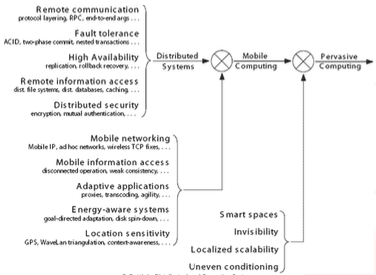
\includegraphics[width = .7\textwidth]{images/lezione1/pervasive-problems.png}
\end{center}
Chi progetta sistemi di pervasive computing deve risolvere tutte le problematiche dei sistemi distribuiti, le problematiche di mobile computing (mobilità dei nodi) e le problematiche tipiche del pervasive computing, come ad esempio smart spaces, invisibility.

Esempi di sistemi distribuiti pervasivi: 
\begin{itemize}
    \item sistemi di ambienti smart: ad esempio un insieme di sensori che ci permette di analizzare il traffico.
    Anche le macchine sono dei sensori: la macchina potrebbe sfruttare la fotografia per vedere quando un semaforo è verde, ma un'applicazione più efficiente potrebbe essere il fatto che il semaforo abbia un sistema integrato che permette di comunicare un segnale quando diventa verde con tutte le auto.
    \item e-health care system: esempio, sistemi in grado di fornire dati rispetto a determinate persone . 
    Un altro impatto dei sistemi pervasivi sulla società riguarda la medicina
\end{itemize} 



\begin{comment}
-------------------
 
Mara Venier

Tutto il materiale è soggetto a copyright, non è autorizzata la diffusione.

Un sistema distribuito è .. Definizione
1. Un sistema fatto di diversi nodi, indipendenti tra loro (ognuno ha architettura classica di computer, non hanno memoria condivisa e sono collegati tra di loro in qualche modo). L'aspetto più importante è che agli utenti appare come un solo sistema.

Da un punto di vista più architetturale, potremmo vederlo così:
Immagine
Ogni computer ha un suo local OS, delle applcazioni che vuole far girare e c'è uno strato di software sopra ai sistemi operativi che fa comunicare le applicazioni (middleware). Un sistema distribuito si ottiene sviluppando un softwre ad un certo livello che fa sembrare il sistema un sistema unico agli utenti.

Esempio 1
Non soltanto i file sono condivisi, ma anche le risorse di calcolo.
Esempio 2
Nei multiplayer online games, uno che gioca non deve sapere dove lo stato del gioco viene memorizzato
Esempio 3
WWW sistema distribuito che si occupa della gestione distribuita di documenti identificati univocamente con URL. Il web non è esattamente un sistema distribuito. Attraverso l'URL si capisce dove si trova il documento, la trasparenza, quindi, è svanita. In un sistema distribuito vero devo avere identificatori di risorse che non danno informazioni sulla locazione dei documenti.

Altra definizione di Leslie Lamport: ....
Un sistema distribuito ideale non dovrebbe mai bloccarsi. Quando succede qualcosa, è difficile capire cosa sia successo. Il debugging in un sistema distribuito è molto difficile. In alcuni casi i problemi sono semplicemente irrisolvibili, non difficili. In particolare, la condizione di consenso. Tutti i partecipanti al sistema siano d'accordo su un certo stato del sistema complessivo. Questi algoritmi funzionano sotto determinte condizioni che a volte non si verificano nell'ambiente reale. Non sono da dare per scontate.

Obbiettivi sistema distribuito:
- rendere risorse accessibili;
- trasparenza (molto importante!), che va a nascondere l'aspetto che sia distribuito
- apertura
- scalabilità

Trasparenza:
- accesso: nasconde differenze di filesystem e/o rapprestanzione dati nell'accesso ad una risorsa condivisa attraverso un'API 
- location: non devo sapere dove la risorsa si trova
- migration: senza che l'utente lo sappia, una risorsa potrebbe spostarsi da un posto all'altro.
- relocation: uguale a sopra, ma mentre è in uso. (?)
- replication: nascondere il fatto che ci siano N copie di una risorsa. N copie perché la ridondanza permette si sopperire a guasti di qualche nodo e per efficienza, ad esempio la locazione geografica potrebbe rendere più rapido l'accesso alla risorsa.
- falire: nascondere i falure e ripristinre automaticamente la risorsa

Implementare meccanismi resistenti al failure è un task molto defficile.

Apertura:
Facilità interoperabilità, portabilità ed estensibilità. Può essere ottenuta con l'uso di protocolli standard, ...

Scalabilità:
Vogliamo che le prestazioni possano migliorare nel momento in cui venga ampliato il sistema. Evitare centralizzazione di servizi, dati e algoritmi.

Un algoritmo centralizzato delega a un nodo il coordinamento del processo. Un algoritmo decentralizzato:

- Nessuna macchina ha lo stato completo del sistema
- ...
- ...
- ... In un sistema distribuito non esiste la coordinazione dei programmi con l'orologio. Ciascun orologio di ciascun nodo rallenta o accellera progressivamente rispetto al tempo di riferimento. Quindi non sono mai sincronizzati perfettamente tra loro. Ci sono algoritmi per cercare di avvicinarsi.

Scalabilità:
In un contesto client/server rendo scalabile il sistema scaricando un po' lavoro lato client. Il server sarà meno carico e con l'aumentare dei client, il sistema è più scalabile.

Un first time developer tende a fare questi errori (assunzioni):
...
...
... homogenous = link hanno più o meno la stessa velocità
...
... 

Da quando è nata, Amazon si è buttata su un'architettura a sistemi distribuiti. Paxos è un algoritmo usatissimo, Google usa delle varianti. Paxos è un algoritmo di consenso, mette d'accordo i nodi circa lo stato di una macchina (?). 

Tipi di sistemi distribuiti
- Computing Systems: ad esempio cloud, cluster (utilizzati dai principali fornitori di cloud, sta anche sotto al cloud).
Cluster: caratterizato da closely connected by high-speed, che garantiscono tempi di latenza controllati e prevedibili, permettendo di fare assunzioni che non si possono fare in generale sui sistemi distribuiti. Obbiettivi: high performance (distribuisce il calcolo su piu nodi) e alta disponibilità (se un sistema va offline, fornisce comunque la richiesta). Due tipi di cluster:
.Asimmetrico: qualche nodo ha un urolo principale rispetto ad altri (nodo master) che distribuisce i task ad un insieme di nodi di compuazione. Esempio Google Bord, sistema utilizzato internamente a Google per gestire i suoi cluster. Beowulf analogo per linux
.Simmetrico: non c'è un master. Questi nodi devono auto-organizzarsi per distribuire il carico e rendere le stesse funzionalità in qualche modo. Ad esempio MOSIX, che ha molteplici versioni, che in ambito linux permette di realizzare cluster simmetrico.
FIGURA ASIMMETRICO
Ciascun nodo ha local OS, collegati da Highspeed network oltre a normale rete. Cluster verrà raggiunto dall'esterno attraverso remote access network. Questi nodi sono tutti uguali, tranne master che ha un applicazione di managemente per distribuire il carico sui nodi.
Esempio di Borg
BorgMaster è il nodo master. Borglet eseguono parti di applicazioni che vengono scaricati sui nodi che partecipano/slave (non master) in modo tale che venga distribuita la computazione, ecc. 
Il master può essere o non essere collegato ad high speed network, poiché la comunicazione piu frequente avviene tra i nodi ed è li che si vuole ottimizzare.
BorgMaster è replicato perché altrimenti se andasse giu il master si bloccherebbe tutto. I dati fondamentali che ha bisogno il master per operare vengono condivisi sulle copie atraverso uno storage distribuito e Paxos garantisce che tutti abbiano la stessa visione sullo stato del sistema.
Da Borg ha preso ispirazione Kubernetes. Sistema di gestione di cluster piu sofisticato (sviluppato da Google). Utilizzato in ambienti cointeinerizzati. Google ha donato questo sistema alla Linux Foundation ed è quindi open source. Etcd è un database chiave valore. Borglet - Kubelet.
Cloud computing
Il cluster assume che le macchine siano localizzate nello stesso posto, per essere collegate ad una rete ad alta velocità. Un'infrastruttura cloud prevede anche distribuzione geografica. Saranno collegate tra loro con canali che utilizzato internet.
Facile acquisire piu risorse, se l'applicazione ne ha bisogno, o usarne di meno, semplicemente (in maniera automatizzata) ri-configuro la macchina e la faccio ripartire (?).
I nodi sono eterogenei. Nei cluster spesso le macchine sono identiche. Nel cloud i nodi possono essere invece molto eterogenei in hw e OS. Anche le network connections sono eterogenee. Possibile ri-configurare in maniera semplice e autonoma le risorse disponibili.
Queste capacità del cloud sono disponibili su tutta la rete accedute da meccanismi standard (trasparenza rispetto all'accesso) tramite API.
Resource pooling: insieme di risorse che mette in comune per gestire le domande di tutti gli utenti.
Elasticità: rapidamente posso dare e restituire risorse.
Chi implementa un cloud deve implementare sistemi di misura. (quanto le risorse sono utilizzate)
Modelli di cloud:
SaaS: un utente inesperto si appoggia ad un software fornito dal cloud.
PaaS: un via di mezzo tra IaaS (ho bisogno una macchina, non la voglio comprare ma voglio autonomia su quello che posso installarci, voglio soltanto l'infrastruttura) e SaaS (?). L'applicazione finale la voglio sviluppare io, però voglio utilizzare db ad alto parallelismo/disponibilità che mi viene fornito. QUindi uso uello del cluster. 
Cloud deployment models:
public
private: faccio usare il mio cloud ad una sola organizzazione.
community: una spece di private in cui diverse organizzazioni si mettono insieme.
hybrid: posso avere sia dati pubblici che privati. Faccio quindi una soluzione ibrida in maniera da integrare, mantenendo un certa località dei dati e controllo di accesso.
Switch per gestire una rete ad altà velocità e tecnologie di load balading hw e sw molto sofisticate.
Ogni data center ha migliaia di nodi collegati tra loro.

-Information systems
-Pervasive systems
Questa classificazione non è esaustiva, in realtà

IOT: dispositivi connessi (possono far parte di sistemi disribuiti) spesso con sensori che producono enormi quantità di dati, alcuni dei quali devono essere processati in tempo reale. Quindi la latenza introdotta dal cloud in molti casi si rivela insufficiente. Quindi l'idea è di avere una struttura gerarchica (anzichè solo cluster dislocati del mondo), in cui abbiamo server vicini a dove i dati vengono prodotti (edge, confine della rete) e questi nodi riescono a connettersi con i dispositivi che producono questi dati e quindi fare processing o preprocessing in tempo reale. In un modo che il cloud generico non riuscerebbe a fare.
5G ha un ruole chiave in questo, ma da solo non riesce. I fornitori di 5g stanno cercando di entrare nel cloud e edge computing, anche perché le reti sono sempre di piu configurate da software e quindi avere un edge server serve anche a gestire meglio la rete e la computazione che deve essere fatta anche a basso livello sulla rete.

I dispositivi di edge possono essere di tipo di verso, ma sostanzialmente sono un primo passaggio da IoT e sensori verso il cloud. Il preprocessing viene fatto nell'edge.

Fog viene usato spesso come sinomino, ma a volte viene utilizzato in maniera differente per indicare i livelli di decentralizzazione in gerarchie a piu di 3 livelli (?).

Information systems
...
In un contesto distribuito, gestire le transazioni è più complicato.

Pervasive computing
Mark Weiser viene considerato un po' un capostipite di questa area di informatica. (?)

L'idea generale è che il calcolo sparisca, nel senso che la trasparenza sia totale. Non dobbiamo andare in giro con i portatili poiché troviamo nell'ambiente qualcosa che fa lo stesos servizio.

Un distributed pervasive system è un sistema distribuit con qualche caratteristica in piu. Ci sono nodi non convenzionali. Oggetti con capacità di calcolo (non fatti esattamente per fare calcolo, spesso per capire o fare cose nell'ambiente). Altra caratteristica, piu difficile da implementare: adattività. Esteso per capire cosa succede nell'ambiente in realtime e avere un effetto sull'ambiente. Da alcuni di questi oggetti riceveremo informazioni che ci possano fare capire (con AI) cosa sta succedendo e si adatterà per are cosa è meglio fare in quel contesto. Quindi ha nodi aggiuntivi e un comportamenteo adattivo. 

Chi deve progettare sistemi di pervasive computer, deve risolvere tutte le problmeatice di distributed systems, le problematiche di mobile computing ( mobilità dei nodi) e cose tipiche di pervasive computing, come smart spaces (dispositivi sensoristici localizzati nello spazio (?)).




Parte dopo fatta a caso, ok? ciao.
Esempi di sistemi distribuiti pervasivi:
...
...
... energy mangement: bisognerà monitorare i consumi. Se riuscissimo a coordinre l'acquisizione di tutti i dati di una città...
Smart trasporation: insieme di sensori ci permettono di analizzare il traffico di un città 


---------------------------------------------------------------
Fabustain

Scalabilità:
Richiesta da browser: indirizzo simbolico -> Interrogato il DNS. 
Errori che si tendono a fare quando si sviluppano sistemi distribuiti:
...
...
L'unico modo per rendere un sistema trasparente e farlo comunicare è quello di mandarsi i messaggi. In un contesto come questo non c'è memoria condivisa. Se c'è è virtuale e costruita da messaggi che si scambiano. Latenza zero dunque non è un'assunzione che può andare bene.

Paxos: usatissimo, anche da amazon. -> Algoritmo di consenso

TIPI DI SISTEMI DISTRIBUITI:
---Computing systems: "Cloud" Ci sono i cluster che sono ampiamente utilizzati dai principali fornitori di cloud. Cluster -> connessione vicina e velocità elevata. Vengono usati per distribuire calcolo su più nodi e alta disponibilità nel caso qualche nodo vada offline.
Due tipi di cluster:
Simmetrico: Non c'è il master. SIstema paritario in cui tutti i nodi hanno lo stesso ruolo. E' più difficile perchè i nodi devono auto-organizarsi per distribuirsi il carico.
Asimmetrico: (più utilizzato). CI sono nodi più importanti di altri. Il master distribuisce i task ad un insieme di nodi di computazione. (Borg, sistema usato da google per gestire i cluster)

Borg: C'è il borg master -> nodo master. I nodi slaves. Una parte dell'applicazione viene scaricata sui Borglet dei nodi slaves. 
Perchè il borg master è replicato più volte nella figura?
E' perchè in un sistema un e si blocca il sistema. I dati che servono al master sono distribuiti su più macchine (store distribuito). Paxos garantisce che tutti i master abbiano la stessa visione sullo stato del sistema.

Kubernetes: Prende ispirazione da Borg, sviluppato da google. Più sofisticato di borg. Sistema per gestire cluster in ambienti containerizzati. Google ha donato questo sistema alla linux foundation. Usato sulle stack open source di cloud computing.

Cloud Computing: Il cluster saranno collegati con canali che potrebbero anche essere dedicati ma spesso sono canali che utilizzano internet. Le asssunzioni di latenza che si fanno sui cluster non si possono fare sul cloud computing. 
...
...
...
...
...
Sistemi di misura: QUando arriva il conto dal provider il conto ti dice quante risorse hai utilizzato.
Modelli del cloud: 
SaaS: Un utente che non dispone di un software tipo GMAIL fa uso di software via cloud
PaaS: 
IaaS:

Private cloud: Ad esempio quello dell'università. Io faccio usare il cloud ad una sola organizzazione.
Community cloud: Private ma con più organizzazioni che si mettono assieme
Public cloud: pubblico
Hybrid Cloud: Dati pubblici e dati privati

Infrastruttura cloud:
Ogni data center ha migliaia di nodi collegati tra di loro

Edge/Fog Computing:
Negli ultimi anni si sono visti un uso massiccio di IoT. Dispositivi connessi che spesso hanno sensori che producono enormi quantità di dati che molte volte devono essere processati in tempo reale e quindi la latenza introdotta dal cloud si dimostra insufficiente. Dunque è megli oavere una struttura gerarchica con server vicini a dove vengono prodotti i dati. I nodi si connettono con i dispositivi che producono i dati e duqnue fanno un pre-processing in tempo reale.
Fog viene usato come sinonimo e a volte in modo differente per indicare che la struttura gerarchica ha più di 3 livelli.

Distribyted information systems:
Sistemi di veicoli autonimi -> Agenti autonomi con ognuno che diventa un nodo. (Droni-robot-metropolitane-perseverance...)
I database di norma sono ottimizzati per lavorare su più nodi.

Pervasive computing
Capostipite "Mark Weiser". Una tecnologia vincente è una tecnologia che utilizziamo senza accorgercene. Se poi sparisce, ci manca. Esempio il google home --> Lo uso senza sapere quello che cè dietro. L'idea è che la trasparenza è importante, totale. L'idea è quella di riuscire ad ottenere la capacità di avere tutte le funzionalità di un pc ovunque.

Nodi non convenzionali: Oggetti con capacità di calcolo (smarphone, smartwatch..). Non sono fatti esattamente per fare calcoli. In generale le applicazioni più importanti dell'iot sono nell'industrial iot.
Un sistema pervasivo deve avere la caratteristica della adattività. L'applicazione deve essere in grado di rispondere a degli eventi in modo adattivo e autonomo. L'adattività può essere banale o sofisticata. Nel parvesing computing si hanno tutte le problematiche del mobile computing, del distributed systems e anche delle cose tipiche del pervasive computing (Eempio non avere interfacce).
Esempi di sistemi distribuiti pervasivi:
Applicazioni per energy managment (sostenibilità). Migliorare il consumo energetico a livello di città/nazione è un problema distribuito pervasivo. Utilizzare i sensori disposti nell'area per analizzare cosa succede in quell'area.
Monitorare il traffico, lo smog etc... Smart cities. (C'entra anche l'edge/fog computing in tutto questo).

E-Health care systems: Utilizzo di sistemi di monitoraggio per migliorare le cure.



---Information systems:
---Pervasion SYstems:



\end{comment}

